\documentclass[11pt]{article}
\usepackage{graphicx}
\usepackage[a4paper, margin=2.5cm]{geometry}
\usepackage{parskip}
\usepackage{hyperref}
\usepackage{bookmark}
\usepackage{titlesec}
\usepackage{float}  
\titleformat{\section}{\large\bfseries}{\thesection.}{1em}{}

\title{SIT102 - HD Report \\ 2D-Platformer Game}
\author{Saatvik Sharma \\ S225158822}
\date{}

\begin{document}
\maketitle
\newpage
\tableofcontents
\newpage


\section{Introduction}

This report is a summary and refelection on my 2d platformer game which is inspired the classical Super Mario game. The game was created using C++ and the SplashKit library tools. The aim of the game is to reach the final flag by going over the platforms and avoiding falling down. If the player reaches the flag, the game is won and player sees the message "You Win!" on the screen, but if player falls down the game is lost and a message shows up showing you lost, but you can always try again by pressing space.



\section{Features and Implemetation}

The game has various features such as player moverment towards left and right on the ground and jumping. There is gravity physics which pulls the player down when it is in the air. Moreover, collisons are detected using AABB (Axis-Aligned Bounding Box) method, which checks if the player is colliding with the ground or the goal post. Moreover, the game simulates level progression by using a invisible goal post which is placed at the end of the level and when that post is reached the platforms are replaced and their coordinates are changed to create a new frame. This can made to look like a continuous level progression by using the same platforms coordinates in ending of previous level and starting of the next level.
Moreover, the game uses variosu UI elements for the paltforms, player, goal post and the ground. The player is drawn using a bitmap image of mario, and it changed according to the action player character is doing. On top of it,the player can reload the game from the very beginning by pression the space key, which resets the game and music plays play throughut the game when the game state is PLAYING.

\section{Evidence of tutor interaction}
\begin{figure}[!ht]
    \centering
    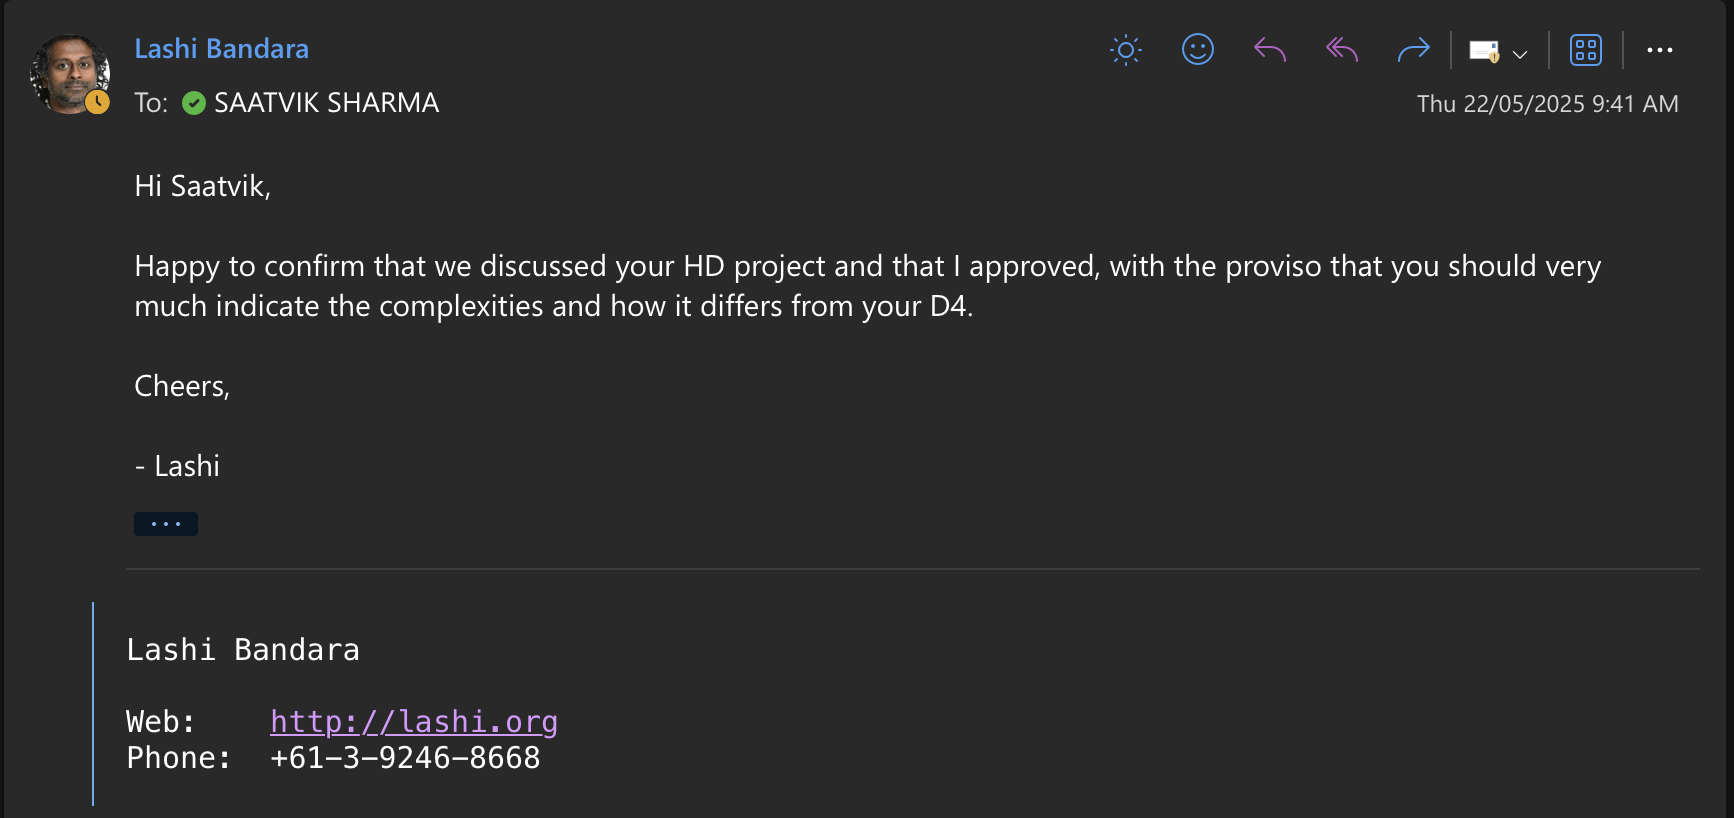
\includegraphics[width=0.8\textwidth]{/Users/rex/Documents/Study_Material/SIT102_Intro_to_programming/H1/Screenshot 2025-05-25 at 21.54.15.png}
    \caption{Screenshot of tutor interaction showing feedback on the game design and implementation.}
\end{figure}

\section{Iterative Development Process}

Before the I made my game for the HD I had to make a small scale program of the game to test the physics engine and the game mechanics. I used simple boxes to represent simpel platforms and the player. But now I used the Bitmap images to make this less tedious and more pleasant to look at. 
\begin{figure}[!ht]
    \centering
    \includegraphics[width=0.8\textwidth]{/Users/rex/Documents/ScreenShots/Screenshot 2025-05-25 at 15.40.47.png}
    \caption{This is the the picture of the the final draw\_game function of the game which implemented the different images for the player(for different action), platforms, background and the goal post.}
\end{figure}

\begin{figure}[!ht]
    \centering
    \includegraphics[width=0.8\textwidth]{/Users/rex/Documents/ScreenShots/Screenshot 2025-05-25 at 22.19.11.png}
    \caption{This is the picture of the final Check\_collisions function which checks for the collisions between the player and the ground, goal post and the platforms. It also checks the level of the game and places the player automatically at the start of the level, giving the illusion of continuous level progression.}
\end{figure}

\begin{figure}[!ht]
    \centering
    \includegraphics[width=0.8\textwidth]{/Users/rex/Documents/ScreenShots/Screenshot 2025-05-25 at 22.22.57.png}
    \caption{This is the picture of the fucntion which loads the level this was an addition to the previous game design which just has one level and the player had to reach the goal post to win. But now when player reaches the goal a new set of platforms and goal is created on the bases of which level the game is currently running on.}
\end{figure}

\begin{figure}[!ht]
    \centering
    \includegraphics[width=0.8\textwidth]{/Users/rex/Documents/ScreenShots/Screenshot 2025-05-25 at 22.32.10.png}
    \caption{ This is the picture of the main funciton of the game which runs the game but there are more things which are added here such as the music which plays throughout the game and the option to reload the game by pressing space key. Which resets the player position, level and the game state.}
\end{figure}

\clearpage
\section{Demonstration Video}

You can watch the demonstration video here: \href{https://youtu.be/boPe4kzw5Eo}{Click to watch on YouTube}.




\end{document}